% Intended LaTeX compiler: pdflatex
\documentclass{llncs}
\usepackage[utf8]{inputenc}
\usepackage[T1]{fontenc}
\usepackage{graphicx}
\usepackage{grffile}
\usepackage{longtable}
\usepackage{wrapfig}
\usepackage{rotating}
\usepackage[normalem]{ulem}
\usepackage{amsmath}
\usepackage{textcomp}
\usepackage{amssymb}
\usepackage{capt-of}
\usepackage{hyperref}
\institute{1337777.OOO}
\titlerunning{Review 1337777.OOO solution programme}
\author{Christopher Mary}
\date{}
\title{Review 1337777.OOO solution programme : Maclane pentagon is some recursive square}
\hypersetup{
 pdfauthor={Christopher Mary},
 pdftitle={Review 1337777.OOO solution programme : Maclane pentagon is some recursive square},
 pdfkeywords={},
 pdfsubject={},
 pdfcreator={Emacs 25.1.2 (Org mode 9.0.3)}, 
 pdflang={English}}
\begin{document}

\maketitle
\begin{abstract}
This memo presents that some random-moment new angle of view, that
Maclane pentagon is some recursive square, onto some decades-old
question may solve some common falsification in mathematics. Moreover
the computational logical content of this new angle of view is
programmed into the COQ computer « 1337777.OOO//coherence2.v » . En
passant, this memo confirms that the only real mathematical research
or industry is the « engineering » of some computational-logical
software with varying degree of embedded logicalness, and everything
else is the education or teaching of « ideas » .
\keywords{associative coherence ; Maclane ; angle of view}
\end{abstract}

\section{Outline}
\label{sec:org0b05bf5}

This memo presents some new lemma, that Maclane pentagon is some
recursive square, which is held in the real deduction of the Maclane
associative coherence, because Maclane's old deduction-attempt is not
the reality. Moreover the computational logical content of this
random-moment new angle of view is programmed into the COQ computer «
google.com/\#q=1337777.OOO//coherence2.v » . This lemma constructs some
adjunction functor from the associative category of words-objects and
bracketing-arrows to the semiassociative (oriented bracketing-arrows)
category. Elsewhere this associative coherence is the meta for the
completeness lemma of another semiassociative coherence which does
lack some more-common Newman-style confluence lemma.

One common way to automatically obtain any adjunction functor is to
start by giving the unit of the adjunction (here the normalization of
words) and by giving the universality-map of this unit of the
adjunction. This new angle of view is that the Maclane pentagon is
precisely one such given half of this universality-map, but it is
sufficient.  As shown in this view :

\begin{figure}\centering 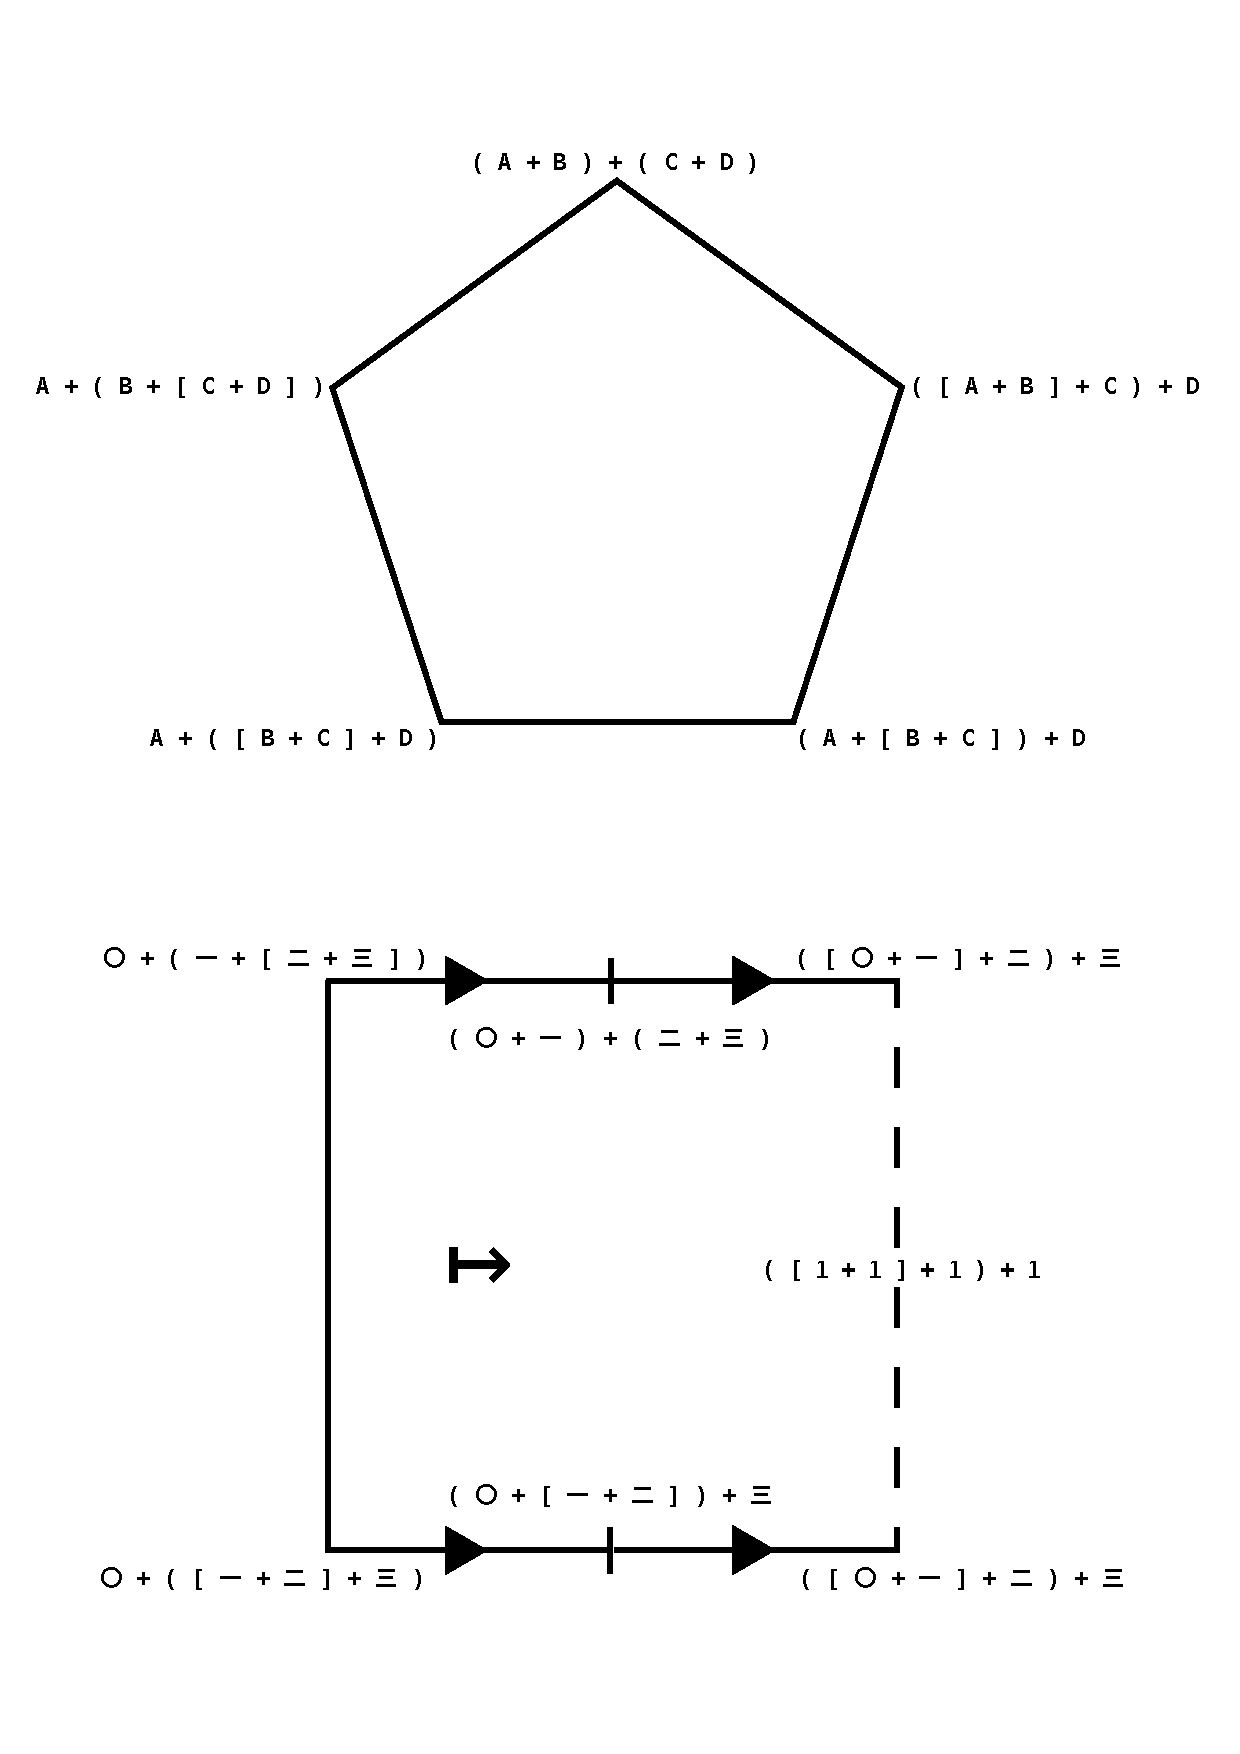
\includegraphics[scale=0.5]{maclaneSolution.svg.pdf} \caption{View}\end{figure}
\end{document}
